\RequirePackage{iftex}\ifPDFTeX\pdfoutput=1\relax\fi
% skycmd methods paper. The text and every number are those of the web page
% site/paper/methods/index.md (https://maxgfr.github.io/skycmd/paper/methods/); when the page
% changes, this file follows it. Built by scripts/build-paper.sh --methods (Tectonic); compiles
% with pdfLaTeX and BibTeX too. The figure, figure-1.tex, is written by
% scripts/paper-methods-figure.py.
\documentclass[11pt]{article}

\usepackage[T1]{fontenc}
\usepackage{newtxtext,newtxmath}
\usepackage[letterpaper,margin=1in]{geometry}
\usepackage{microtype}
\usepackage{amsmath}
\usepackage{array,booktabs,tabularx}
\usepackage{enumitem}
\usepackage{xcolor}
\usepackage{tikz}
\usepackage{algorithm}
\usepackage{algpseudocode}
\usepackage[numbers,sort&compress]{natbib}
\usepackage{caption}
\usepackage{fancyvrb}
\usepackage{xurl}
\definecolor{linkblue}{rgb}{0.10,0.25,0.55}
\usepackage[colorlinks=true,linkcolor=linkblue,citecolor=linkblue,urlcolor=linkblue,
  pdftitle={Small ternary decision models trained on one laptop: architecture, training,
  closed-loop calibration and a Rust engine for the browser},pdfauthor={Maxime Golfier}]{hyperref}

\captionsetup{font=small,labelfont=bf,labelsep=period,skip=6pt}
\captionsetup[table]{position=top}
\setlist{itemsep=2pt,topsep=4pt,parsep=0pt}
\setlength{\emergencystretch}{2em}
\newcolumntype{L}{>{\raggedright\arraybackslash}X}
\newcolumntype{P}[1]{>{\raggedright\arraybackslash}p{#1}}
\newcolumntype{R}[1]{>{\raggedleft\arraybackslash}p{#1}}
\renewcommand{\arraystretch}{1.15}
\renewcommand{\algorithmicrequire}{\textbf{Input:}}
\urlstyle{same}

\title{Small ternary decision models trained on one laptop:\\
architecture, training, closed-loop calibration\\
and a Rust engine for the browser}
\author{Maxime Golfier\\[2pt]
\normalsize\url{https://github.com/maxgfr/skycmd}}
\date{21 November 2026}

\begin{document}

\maketitle

\begin{abstract}
\noindent This report describes how the models of the skycmd project are built, trained, calibrated and run, precisely enough to reimplement them; a companion report~\cite{golfier2026skycmd} holds the protocol and every gate as read. The models answer typed questions (\texttt{choice}, \texttt{score} and \texttt{noul}) about a state, with a probability for every option in one forward pass. The graph encodes the question and its options once and caches them, encodes each new state with one token per measured value, loops a small stack of shared blocks with an exit after each pass, and scores every option with a fusion head in which no option sees another. Every linear layer is ternary, trained with a straight-through estimator after a float warm-up and stored at 2 bits per weight: s3-pico holds 445,345 parameters in 251,104 bytes. Training mixes game oracles written in Rust, public data sets and soft labels from an open-weight teacher, puts a loss on every exit, and runs DAgger on the games, under budgets counted in working minutes on one Apple M5 laptop. Exit thresholds are chosen by playing the games, because thresholds fitted on held-out questions made s2-nano crash in every Flappy episode. Variants of the same blocks detect the end of a turn in speech, route requests to tools, judge secret candidates proposed by rules, and forecast time series. One Rust engine runs every file natively and in WebAssembly, where s6-nano's probabilities differ from the native ones by at most 9.5e-7 on 200 bench questions. Most pieces are adopted from prior work, and the report says which; what it adds is their combination in files of a few hundred kilobytes, the closed-loop check of the exits, and the measurements.
\end{abstract}

\begin{center}
\fbox{\parbox{\dimexpr\linewidth-2\fboxsep-2\fboxrule\relax}{\small
\textbf{Technical report, not peer-reviewed.} This report has not been peer-reviewed, nor reviewed by anyone outside the project. Every number in it is copied from a page or a file of the repository, and each one links to its evidence. Where a number is computed here, the text says so. It describes the methods; the protocol and every gate's reading are in the companion report~\cite{golfier2026skycmd}.
The web version of this report is at \url{https://maxgfr.github.io/skycmd/paper/methods/}.}}
\end{center}

\section{Introduction}\label{sec:1}

A \emph{decision model} receives a state (a game frame, a short text, the last seconds of audio) and one or more typed questions, and returns a probability for every allowed option in one forward pass, without generating text. A \texttt{choice} question picks one of several named options, a \texttt{score} question one of several ordered levels, and a \texttt{noul} question is a probabilistic yes or no (\href{https://github.com/maxgfr/skycmd/blob/main/docs/SPEC.md}{\texttt{docs/\allowbreak{}SPEC.md}}). TypeSafe introduced this format with its closed model Jev~\cite{jev}, and open models now serve it from 706,048 parameters for one form-filling task~\cite{cua} to 421M~\cite{laya}.

skycmd trained such models from scratch under three constraints: small files, from 142,912 bytes to 3,692,288 bytes for the s6 family and most of them under one megabyte (\href{https://maxgfr.github.io/skycmd/models/manifest.json}{manifest}); one Apple M5 laptop with 16 GB of memory, the machine its owner works on, for every run (\href{https://github.com/maxgfr/skycmd/blob/main/docs/big-run-report.md}{\texttt{docs/\allowbreak{}big-run-report.md}}); and the browser, where every demo runs the file its numbers were measured on.

The companion report~\cite{golfier2026skycmd} is the record of the protocol and of every gate's reading. This report is its counterpart on method: it describes what the code does, gives at most one sentence per system on its result, with a pointer, and follows the code where the project's specifications disagree with it.

It contributes five descriptions, each with the parts it adopts named as such.

\begin{enumerate}
\item \textbf{The decision graph} (section~\ref{sec:3}): two streams and a cache, options isolated by the attention mask, one token per measured value, shared blocks looped with an exit after each pass, a fusion head shared by the exits, and ternary weights trained in. Each piece is adopted: order invariance from Set-LLM~\cite{egressy2025setllm} and Amit~\cite{amit2026permutation}, a looped shared block with an answer after each loop from TRM~\cite{jolicoeur2025trm} and Ouro~\cite{zhu2025ouro}, one token per value from FT-Transformer~\cite{gorishniy2021ftt} and FoNE~\cite{zhou2025fone}, ternary weights from BitNet b1.58~\cite{ma2024bitnet}. Built from them, s3-pico is the smallest open model we found that covers the whole typed format, and the only ternary one (\href{https://maxgfr.github.io/skycmd/novelty/\#_1-a-decision-model-in-251-kb}{What we bring, section 1}).
\item \textbf{A training recipe for one laptop} (section~\ref{sec:4}): masked-language pretraining with a loss on numbers, a loss at every exit, soft labels from an open-weight teacher kept only where they agree with the gold answer, DAgger~\cite{ross2011dagger} on the games, and budgets counted in working minutes. A recipe table gives the settings of seven published files.
\item \textbf{Exit thresholds chosen by playing} (section~\ref{sec:5}): temperatures per exit, type and bucket, and a threshold accepted only if the games played at that threshold stay within 2\% of full depth. Choosing exit thresholds against the task's own success is what DeeR-VLA does~\cite{yue2024deer}; the readings here confirm that line of work and do not introduce it. A conformal variant is described with the reason it was rejected.
\item \textbf{Task-specific systems on the same blocks} (section~\ref{sec:6}): an end-of-turn student of a larger audio model, a tool router fused with a static embedding, a verifier of secret candidates, and a forecaster. The verifier's design, rules that propose and a learned model that judges, is that of Samsung's CredSweeper~\cite{credsweeper} and GitGuardian's FP Remover~\cite{fpremover}.
\item \textbf{One inference engine in Rust} (section~\ref{sec:7}): the GGUF files, the ternary kernels, the caches and the WebAssembly builds, with the measured agreement between the browser and the native engine.
\end{enumerate}

What the combination adds is a chain from data to a browser in which every step fits one laptop and every claim is measured; no single piece is new (\href{https://maxgfr.github.io/skycmd/novelty/\#at-a-glance}{What we bring}).

\section{Related work}\label{sec:2}

The references are those of the companion report, which checked each one against its arXiv or project page; the project's \href{https://maxgfr.github.io/skycmd/sources/}{Sources} page lists them all.

\textbf{Decision models.} Jev~\cite{jev} launched the format; Laya~\cite{laya} and oscar-1-17m~\cite{oscar} are open models in it on pretrained encoders, and two smaller ones appeared in 2026: cua-s1-forms~\cite{cua}, a byte-level encoder of width 128 for one form-filling task, and TinyDecide~\cite{tinydecide}, fine-tuned from ELECTRA-small. The models of this report are trained from scratch.

\textbf{Options, depth and exits.} Set-LLM~\cite{egressy2025setllm} and Amit~\cite{amit2026permutation} isolate the options from one another, and Jeva~\cite{li2026jeva}, concurrent work, also reuses their representations across requests. Weight sharing across depth goes back to Universal Transformers~\cite{dehghani2019ut}; a loss at every exit follows deeply-supervised nets~\cite{lee2014dsn}, and skipping loops at random in training follows stochastic depth~\cite{huang2016stochastic}. Early exits go back to BranchyNet~\cite{teerapittayanon2017branchynet}, DeeBERT~\cite{xin2020deebert} and FastBERT~\cite{liu2020fastbert}. Conformal risk control~\cite{angelopoulos2022crc} gives exit thresholds a guarantee, in the setting of CALM~\cite{schuster2022calm} and Fast yet Safe~\cite{jazbec2024fastyetsafe}, and DeeR-VLA~\cite{yue2024deer} sets the exit thresholds of a robot policy against task success.

\textbf{Weights and training.} Ternary weights at small scale are studied by Nielsen et al.~\cite{nielsen2024bits}, and the encoder block keeps the layout of ModernBERT~\cite{warner2024modernbert}. Temperature scaling and the expected calibration error with 15 equal-width bins are those of Guo et al.~\cite{guo2017calibration}; learning a teacher's soft labels is knowledge distillation~\cite{hinton2015distilling}. The code includes the Muon optimizer~\cite{jordan2024muon}; that its gains over AdamW shrink once AdamW is tuned as carefully~\cite{wen2025optimizers}, and that AdamW can win at equal time on small models~\cite{akhtar2026muon}, is what the project's ablation found too (section~\ref{sec:4.4}).

\textbf{Task-specific work.} The closest small end-of-turn work found is a 1.14M-parameter model distilled into an MFCC-based student~\cite{helwani2026eot}. Routing by embedding similarity is the method of semantic-router~\cite{semrouter}, and the router's lexical score is BM25~\cite{robertson2009bm25}. The verifier is trained on Samsung's CredData~\cite{creddata}. Fracast-0~\cite{zhan2026fracast} is a smaller forecaster that, by its abstract, does better than the one here. Training in Rust and running in WebAssembly is also done by frameworks such as Burn~\cite{burn}; the teachers and baselines of each system are cited in section~\ref{sec:6}.

\section{The decision model}\label{sec:3}

Figure~\ref{fig:1} shows the graph, \texttt{skycmd-s2} in the files, used by s3-pico, s6-nano, s6-micro and the s6 specialists. The training graph is \href{https://github.com/maxgfr/skycmd/blob/main/crates/sky-train/src/s2/model.rs}{\texttt{crates/\allowbreak{}sky-train/\allowbreak{}src/\allowbreak{}s2/\allowbreak{}model.rs}} and the inference graph \href{https://github.com/maxgfr/skycmd/blob/main/crates/sky-infer/src/s2/model.rs}{\texttt{crates/\allowbreak{}sky-infer/\allowbreak{}src/\allowbreak{}s2/\allowbreak{}model.rs}}; the specifications are \href{https://github.com/maxgfr/skycmd/blob/main/docs/SPEC-S2.md}{\texttt{docs/\allowbreak{}SPEC-S2.md}}, \href{https://github.com/maxgfr/skycmd/blob/main/docs/SPEC-S3.md}{\texttt{docs/\allowbreak{}SPEC-S3.md}} and \href{https://github.com/maxgfr/skycmd/blob/main/docs/SPEC-S6.md}{\texttt{docs/\allowbreak{}SPEC-S6.md}}.

\begin{figure}[htbp]
\centering
% The architecture figure of the methods paper, written by scripts/paper-methods-figure.py
% from the same coordinates as site/public/paper/methods/figure-1.svg. Do not edit by hand.
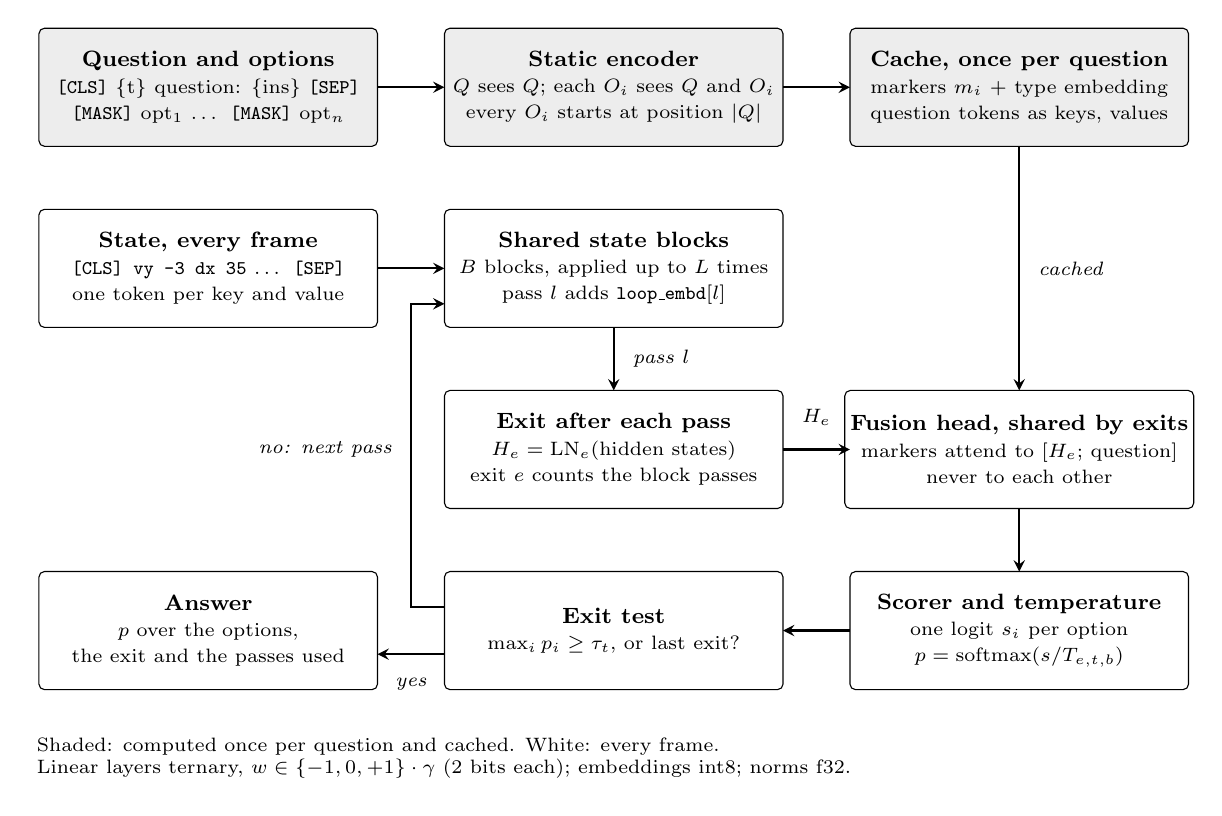
\begin{tikzpicture}[x=1cm,y=1cm,>=stealth,font=\footnotesize,box/.style={draw,rounded corners=2pt,minimum width=4.30cm,minimum height=1.50cm,align=center,inner sep=2pt}]
\node[box,fill=black!7] (in_q) at (2.30,8.50) {\textbf{Question and options}\\{\scriptsize \texttt{[CLS]} \{t\} question: \{ins\} \texttt{[SEP]}}\\{\scriptsize \texttt{[MASK]} opt$_1$ \ldots{} \texttt{[MASK]} opt$_n$}};
\node[box,fill=black!7] (static) at (7.45,8.50) {\textbf{Static encoder}\\{\scriptsize $Q$ sees $Q$; each $O_i$ sees $Q$ and $O_i$}\\{\scriptsize every $O_i$ starts at position $|Q|$}};
\node[box,fill=black!7] (cache) at (12.60,8.50) {\textbf{Cache, once per question}\\{\scriptsize markers $m_i$ + type embedding}\\{\scriptsize question tokens as keys, values}};
\node[box] (in_s) at (2.30,6.20) {\textbf{State, every frame}\\{\scriptsize \texttt{[CLS] vy -3 dx 35} \ldots{} \texttt{[SEP]}}\\{\scriptsize one token per key and value}};
\node[box] (loop) at (7.45,6.20) {\textbf{Shared state blocks}\\{\scriptsize $B$ blocks, applied up to $L$ times}\\{\scriptsize pass $l$ adds \texttt{loop\_embd}$[l]$}};
\node[box] (exit) at (7.45,3.90) {\textbf{Exit after each pass}\\{\scriptsize $H_e = \mathrm{LN}_e(\text{hidden states})$}\\{\scriptsize exit $e$ counts the block passes}};
\node[box] (fusion) at (12.60,3.90) {\textbf{Fusion head, shared by exits}\\{\scriptsize markers attend to $[H_e;\,\text{question}]$}\\{\scriptsize never to each other}};
\node[box] (score) at (12.60,1.60) {\textbf{Scorer and temperature}\\{\scriptsize one logit $s_i$ per option}\\{\scriptsize $p = \mathrm{softmax}(s / T_{e,t,b})$}};
\node[box] (test) at (7.45,1.60) {\textbf{Exit test}\\{\scriptsize $\max_i p_i \geq \tau_t$, or last exit?}};
\node[box] (answer) at (2.30,1.60) {\textbf{Answer}\\{\scriptsize $p$ over the options,}\\{\scriptsize the exit and the passes used}};
\draw[->,thick] (4.450,8.500) -- (5.300,8.500);
\draw[->,thick] (9.600,8.500) -- (10.450,8.500);
\draw[->,thick] (12.600,7.750) -- (12.600,4.650);
\node[anchor=west,font=\scriptsize\itshape] at (12.720,6.200) {cached};
\draw[->,thick] (4.450,6.200) -- (5.300,6.200);
\draw[->,thick] (7.450,5.450) -- (7.450,4.650);
\node[anchor=west,font=\scriptsize\itshape] at (7.570,5.050) {pass $l$};
\draw[->,thick] (9.600,3.900) -- (10.450,3.900);
\node[anchor=south,font=\scriptsize\itshape] at (10.025,4.080) {$H_e$};
\draw[->,thick] (12.600,3.150) -- (12.600,2.350);
\draw[->,thick] (10.450,1.600) -- (9.600,1.600);
\draw[->,thick] (5.300,1.300) -- (4.450,1.300);
\node[anchor=north,font=\scriptsize\itshape] at (4.875,1.120) {yes};
\draw[->,thick] (5.300,1.900) -- (4.875,1.900) -- (4.875,5.750) -- (5.300,5.750);
\node[anchor=east,font=\scriptsize\itshape] at (4.755,3.900) {no: next pass};
\node[anchor=south west,font=\scriptsize,align=left] at (0.00,-0.40) {Shaded: computed once per question and cached. White: every frame.\\Linear layers ternary, $w \in \{-1, 0, +1\}\cdot\gamma$ (2 bits each); embeddings int8; norms f32.};
\end{tikzpicture}

\caption[The decision graph.]{The decision graph. The question and its options are encoded once and cached (shaded); each frame, the state goes through $B$ shared blocks up to $L$ times, and after each pass an exit feeds the fusion head, which is shared by all exits. The answer is returned at the first exit whose top probability reaches the threshold of the question's type, or at the last. The figure is written by \href{https://github.com/maxgfr/skycmd/blob/main/scripts/paper-methods-figure.py}{\texttt{scripts/\allowbreak{}paper-methods-figure.py}}; its text alternative is in the SVG.}\label{fig:1}
\end{figure}

\subsection{Requests and tokenization}\label{sec:3.1}

A request holds a state and one or more questions; a question has a type, an instruction and its options. The options are rendered as Laya's runtime and llama.cpp's server render them: a \texttt{choice} option is \texttt{key} or \texttt{key: description}, a \texttt{score} option is \texttt{level i: description} for i = 0, 1, and so on, and the two \texttt{noul} options are \texttt{false: \ldots{}} and \texttt{true: \ldots{}}, with the defaults \texttt{no, the statement does not hold} and \texttt{yes, the statement holds} (\href{https://github.com/maxgfr/skycmd/blob/main/crates/sky-infer/src/prompt.rs}{\texttt{crates/\allowbreak{}sky-infer/\allowbreak{}src/\allowbreak{}prompt.rs}}).

The tokenizers are byte-level BPE in the GPT-2 style with an NFC normaliser, trained with Hugging Face \texttt{tokenizers} at 1,024, 2,048 or 4,096 entries on the text the model will read: each question head, each option with its leading space, and each state (\href{https://maxgfr.github.io/skycmd/tutorial/07-tokenizer}{tutorial, chapter 07}). Their special tokens have fixed ids: \texttt{[PAD]} 0, \texttt{[UNK]} 1, \texttt{[CLS]} 2, \texttt{[SEP]} 3, \texttt{[MASK]} 4 and \texttt{[NUM]} 5 (\href{https://github.com/maxgfr/skycmd/blob/main/docs/SPEC-S2.md}{\texttt{docs/\allowbreak{}SPEC-S2.md}} §2). A small vocabulary keeps the embedding table close to the size of the network; the game generators clamp their values to small ranges for the same reason.

\subsection{One token per measured value}\label{sec:3.2}

Before BPE, every match of \texttt{-?\textbackslash{}d+(?:\textbackslash{}.\textbackslash{}d+)?} on ASCII digits is replaced by \texttt{[NUM]} and its value is kept in a parallel array, unless the match is glued to a preceding ASCII letter, as in \texttt{b2} or \texttt{glm-5} (\href{https://github.com/maxgfr/skycmd/blob/main/crates/sky-infer/src/num.rs}{\texttt{crates/\allowbreak{}sky-infer/\allowbreak{}src/\allowbreak{}num.rs}}). With \texttt{fuse\_\allowbreak{}numbers}, set in every published s3 and s6 decision file, a \texttt{[NUM]} is removed and its value moved onto the token before it, unless that token is \texttt{[CLS]}, \texttt{[SEP]} or \texttt{[MASK]} or already carries a value; then the \texttt{[NUM]} stays a token of its own. A pair such as \texttt{vy -3} is then one token. The merge happens before truncation, so every window counts merged tokens (\href{https://github.com/maxgfr/skycmd/blob/main/crates/sky-train/src/s2/data.rs}{\texttt{crates/\allowbreak{}sky-train/\allowbreak{}src/\allowbreak{}s2/\allowbreak{}data.rs}}). The embedding of token \emph{i}, whose id is $\mathrm{id}_{i}$, whose value is $v_{i}$ and whose flag $h_{i}$ is 1 when it carries a value, is

\begin{equation}\label{eq:1}
\begin{gathered}
u(v) = \operatorname{sign}(v)\,\ln(1 + |v|), \qquad \omega_k = 2^k \pi / 8, \quad k = 0, \dots, 7,\\
\varphi(v) = \bigl[\, u,\ \sin(\omega_0 u), \dots, \sin(\omega_7 u),\ \cos(\omega_0 u), \dots, \cos(\omega_7 u) \,\bigr] \in \mathbb{R}^{17},\\
e_i = E[\mathrm{id}_i] + h_i \cdot \bigl( W_{\mathrm{num}}\, \varphi(v_i) + b_{\mathrm{num}} \bigr), \qquad W_{\mathrm{num}} \in \mathbb{R}^{d \times 17}.
\end{gathered}
\end{equation}

The signed logarithm compresses magnitudes, and the eight frequencies give periods from 16 down to 1/8 in \emph{u} (computed here from $\omega_{k}$), so nearby values get nearby embeddings and orders of magnitude stay apart; the engine computes the sixteen sines and cosines from one pair by double-angle steps. On the Flappy state used by the benchmarks, value fusion gives 9 tokens instead of 16, \texttt{[CLS]} and \texttt{[SEP]} included (\href{https://github.com/maxgfr/skycmd/blob/main/BENCH.md}{\texttt{BENCH.md}}, section ``Inference'').

\subsection{Two streams, a cache and isolated options}\label{sec:3.3}

The \textbf{static stream} holds the question and its options. Its tokens are Q = \texttt{[CLS]} \texttt{\{t\} question: \{ins\}} \texttt{[SEP]}, followed for each option \emph{i} by $O_{i}$ = \texttt{[MASK]} \texttt{ \{option\}}, with no final separator. The attention mask lets Q attend to Q and each $O_{i}$ attend to Q and to itself only. Positions for the rotary embedding are 0 to |Q| $-$ 1 for Q, and every option starts again at |Q|, so each option's \texttt{[MASK]} marker sits at the same position. Each option is cut to its marker and 48 tokens; if the options leave less than 16 tokens of the head window, every option is cut to max(4, (max\_head $-$ 16) / n) tokens, and the question keeps at least 8 (\href{https://github.com/maxgfr/skycmd/blob/main/crates/sky-infer/src/s2/prompt.rs}{\texttt{crates/\allowbreak{}sky-infer/\allowbreak{}src/\allowbreak{}s2/\allowbreak{}prompt.rs}}). The static encoder's output at each marker is the option's marker vector $m_{i}$, and its outputs at all |Q| question positions, \texttt{[CLS]} and \texttt{[SEP]} included, are the question tokens.

Since no option attends to another and all sit at the same positions, permuting the options permutes the marker vectors and, through the head of section~\ref{sec:3.5}, the probabilities. This holds by construction, as in the prior work of section~\ref{sec:2}; on the s2 models, permuting the options moved no probability by more than 3e-6 on the CPU (\href{https://github.com/maxgfr/skycmd/blob/main/BENCH.md}{\texttt{BENCH.md}}, section ``s2 training runs'').

The \textbf{state stream} is \texttt{[CLS]} state \texttt{[SEP]}, at most max\_state tokens, at positions 0 to S $-$ 1, with full bidirectional attention. It does not see the question, so one encoding of a state serves every question asked about it, such as the action and danger questions of one Flappy frame.

The engine keeps an LRU \textbf{cache} of 16 static streams, keyed by type, instruction and options. An entry holds the marker vectors, the keys and values of the question tokens for every fusion block, and the first fusion block's queries with their attention over the question tokens already computed. A second cache of 4 entries, keyed by the state text, keeps the exits already computed for a state (\href{https://github.com/maxgfr/skycmd/blob/main/crates/sky-infer/src/s2/engine.rs}{\texttt{crates/\allowbreak{}sky-infer/\allowbreak{}src/\allowbreak{}s2/\allowbreak{}engine.rs}}). In a game, the same questions come back every frame, so only the state is new.

\subsection{Shared blocks, loops and exits}\label{sec:3.4}

Both encoders are built from one kind of block. It applies a LayerNorm without bias ($\varepsilon$ = 1e-5), a fused query, key and value projection without bias, rotary embeddings in the rotate-half form with $\theta$ = 10,000 on queries and keys, scaled dot-product attention and an output projection without bias; then a second LayerNorm and a GeGLU feed-forward, [$u_{1}$ | $u_{2}$] = $W_{\mathrm{up}}$ LN(x) with $W_{\mathrm{up}}$ of shape 2ff $\times$ d, x $\gets$ x + $W_{\mathrm{down}}$ (gelu($u_{1}$) $\odot$ $u_{2}$). As in ModernBERT~\cite{warner2024modernbert}, the first block of each encoder has no attention norm on its first application. The number of heads is set per file, or d / 64 by default.

The state encoder has B distinct blocks applied in order, and the sequence is repeated L times. From the second loop on, block 0 normalises its input with a norm of its own, and before loop \emph{l} $\geq$ 1 (counted from 0) a learned loop embedding loop\_embd[\emph{l}] is added to every hidden state, so the shared block knows which pass it is in. Exits sit after given numbers of block passes; exit \emph{e} normalises the hidden states with its own LayerNorm and gives $H_{e}$. s3-pico has B = 1, L = 4 and exits after passes 1 to 4; s6-nano B = 2, L = 2 and exits after 1 to 4; s6-micro B = 2, L = 3 and exits after 2, 4 and 6 (\href{https://github.com/maxgfr/skycmd/tree/main/configs}{\texttt{configs/\allowbreak{}}}). The static encoder is a plain stack of 1 or 2 blocks with a final norm.

\subsection{Fusion head, scorer and probabilities}\label{sec:3.5}

The fusion head turns each option's marker into a score, once per exit, with the same weights for every exit. Each option starts from $x_{i}$ = $m_{i}$ + type\_embd[t], its marker plus an embedding of the question's type. Each of the 2 fusion blocks applies a cross-attention whose queries are the options and whose keys and values are [$H_{e}$; question tokens], the state after exit \emph{e} followed by the cached question tokens; then a ReLU feed-forward of width 2d. Every LayerNorm and linear layer of the head has a bias, and there is no rotary embedding. The options attend to the state and the question, never to each other. The scorer gives one logit per option and the probabilities follow:

\begin{equation}\label{eq:2}
s_i = w_{\mathrm{o}} \cdot \mathrm{gelu}\bigl(W_{\mathrm{c}}\, \mathrm{LN}(x_i) + b_{\mathrm{c}}\bigr) + b_{\mathrm{o}}, \qquad
p^{(e)}_i = \frac{\exp(s_i / T)}{\sum_j \exp(s_j / T)}, \qquad T = T_{e,\,t,\,b(n)}.
\end{equation}

The temperature depends on the exit \emph{e}, the type \emph{t} and the bucket \emph{b}(\emph{n}) of the number of options \emph{n}: 2 or fewer, 3 to 5, 6 to 10, or 11 and more (section~\ref{sec:5.1}). The engine looks up the temperature of (exit, type, bucket), then (exit, type), then (type, bucket), then the type, and uses 1 when none is stored; the training code has only the first two levels (\href{https://github.com/maxgfr/skycmd/blob/main/crates/sky-infer/src/s2/mod.rs}{\texttt{crates/\allowbreak{}sky-infer/\allowbreak{}src/\allowbreak{}s2/\allowbreak{}mod.rs}}, \href{https://github.com/maxgfr/skycmd/blob/main/crates/sky-train/src/s2/config.rs}{\texttt{crates/\allowbreak{}sky-train/\allowbreak{}src/\allowbreak{}s2/\allowbreak{}config.rs}}). The answer depends on the type (\href{https://github.com/maxgfr/skycmd/blob/main/crates/sky-infer/src/engine.rs}{\texttt{crates/\allowbreak{}sky-infer/\allowbreak{}src/\allowbreak{}engine.rs}}):

\begin{equation}\label{eq:3}
\begin{gathered}
\text{choice: } \arg\max_i p_i, \text{ with confidence } \max\bigl(0,\ (p_{\max} - 1/n)/(1 - 1/n)\bigr);\\
\text{score: the expected level } \textstyle\sum_i i \cdot p_i \text{ over the levels } i = 0, \dots, n - 1; \qquad \text{noul: } p_1, \text{ the probability of \texttt{true}.}
\end{gathered}
\end{equation}

At inference the exits run in order, and the engine answers at

\begin{equation}\label{eq:4}
e^{*} = \min\Bigl(\bigl\{\, e : \max_i p^{(e)}_i \geq \tau_t \,\bigr\} \cup \{E\}\Bigr),
\end{equation}
where \emph{E} is the last exit and $\tau_{t}$ is one threshold per question type, shared by all exits; the test uses the calibrated probabilities (\href{https://github.com/maxgfr/skycmd/blob/main/crates/sky-infer/src/s2/engine.rs}{\texttt{crates/\allowbreak{}sky-infer/\allowbreak{}src/\allowbreak{}s2/\allowbreak{}engine.rs}}). A file without a threshold reads 0.9. A threshold of 1 makes the engine start directly at the last exit, so the earlier exits are not computed; the s6 files that the manifest marks as published at full depth store 1 for each type (section~\ref{sec:5.4}). The answer reports the exit and the number of block passes used.

\subsection{Ternary weights, trained in}\label{sec:3.6}

Every linear layer of the encoders and of the fusion head is ternary, and so is the scorer's hidden layer. For a weight matrix W, row \emph{r} is quantized with its own scale:

\begin{equation}\label{eq:5}
\gamma_r = \max\Bigl(\tfrac{1}{k}\textstyle\sum_j |W_{rj}|,\ 10^{-8}\Bigr), \qquad
\hat W_{rj} = \gamma_r \cdot \mathrm{clip}\bigl(\mathrm{round}(W_{rj} / \gamma_r), -1, 1\bigr), \qquad
W_{\mathrm{used}} = W + \mathrm{sg}(\hat W - W),
\end{equation}
where \emph{k} is the number of columns and sg stops the gradient: the forward pass uses $\hat W$, and the gradient reaches the float master weights W unchanged, the straight-through estimator (\href{https://github.com/maxgfr/skycmd/blob/main/crates/sky-train/src/s2/model.rs}{\texttt{crates/\allowbreak{}sky-train/\allowbreak{}src/\allowbreak{}s2/\allowbreak{}model.rs}}). The scale is the mean absolute value (absmean) as in BitNet b1.58~\cite{ma2024bitnet}, but per output row rather than per tensor. The scorer's output layer, the value projection $W_{\mathrm{num}}$, the type and loop embeddings, the norms and the biases stay in float. The token embedding is trained in float and stored in int8 at export, with one scale per row, max |row| / 127; it is not simulated in training (\href{https://github.com/maxgfr/skycmd/blob/main/crates/sky-train/src/s2/gguf.rs}{\texttt{crates/\allowbreak{}sky-train/\allowbreak{}src/\allowbreak{}s2/\allowbreak{}gguf.rs}}).

Quantization starts when the training progress, measured in working time over the budget or in steps, reaches 1 $-$ q, where q is the fraction of the run in QAT. The scripts pass q = 0.9, a float warm-up of 10\%, for a model's first decision training, and q = 1.0, every step ternary, for the DAgger rounds; the command-line default, q = 0.3, is the one of the first specification (\href{https://github.com/maxgfr/skycmd/blob/main/scripts/train-s6.sh}{\texttt{scripts/\allowbreak{}train-s6.sh}}). At the switch the trainer validates both forms, saves the float weights, and leaves the learning-rate schedule as it is. Why train the ternary weights rather than round a float model: on the s2 models, ternarizing without QAT cost 6 to 11 points of validation accuracy (pico 0.470 to 0.406, nano 0.542 to 0.432), and 30\% of the budget in QAT recovered it (pico 0.482, nano 0.556) (\href{https://github.com/maxgfr/skycmd/blob/main/BENCH.md}{\texttt{BENCH.md}}, section ``s2 training runs'').

In the file, each ternary matrix X becomes \texttt{X.tq}, bytes of type I8 holding 4 weights each, 2 bits per weight from the least significant bits up (00 for 0, 01 for +1, 10 for $-$1; 11 is rejected), each row padded to a multiple of 4 weights, and \texttt{X.scale}, one 16-bit float per row. Everything else is stored in 32-bit float. This is how s3-pico's 445,345 parameters take 251,104 bytes, against 1.8 MB in 32-bit float (\href{https://github.com/maxgfr/skycmd/blob/main/BENCH.md}{\texttt{BENCH.md}}, section ``skycmd-s3'').

\subsection{What the published decision files do not use}\label{sec:3.7}

Some options of the code are in no published decision file. \emph{Temporal carry} adds to each frame's state embedding g $\odot$ LN(h), with h the previous frame's final latent and the gate g starting at 0; on s3-pico it did not reduce the depth used and was not shipped (\href{https://github.com/maxgfr/skycmd/blob/main/BENCH.md}{\texttt{BENCH.md}}, section ``Temporal recursion''). \emph{Parallax} and \emph{exclusive self-attention} change the encoder's attention; the ablation of section~\ref{sec:4.4} adopted neither, so every trained s6 file has plain softmax attention, though some configuration files still say \texttt{"parallax": true} before the recipe script overwrites it (\href{https://github.com/maxgfr/skycmd/blob/main/scripts/s6-adopt.py}{\texttt{scripts/\allowbreak{}s6-adopt.py}}). The fast-weight memory is in section~\ref{sec:6.5}.

\section{Training}\label{sec:4}

\subsection{Data}\label{sec:4.1}

\textbf{Game oracles.} Four games are written in Rust: Flappy Drone, Rescue Run, Obstacle Dodge and a Doom-like game (\href{https://github.com/maxgfr/skycmd/tree/main/crates/sky-games}{\texttt{crates/\allowbreak{}sky-games/\allowbreak{}}}). Each writes its state as short \texttt{key value} pairs of small binned integers and computes the useful relations in code: Flappy gives the room above and below the drone rather than absolute heights, so the model maps measurements to a decision (\href{https://maxgfr.github.io/skycmd/tutorial/20-dagger-lessons}{tutorial, chapter 20}). An exact oracle gives a target distribution over the options at every decision. The generator draws an exploration rate per episode from 0, 0.05, 0.15 and 0.3, caps Flappy episodes at 12 pipes, sends 30\% of the records to each game's secondary question, keeps records with a probability that balances the classes, renders the option keys with random synonyms, and splits by episode seed (\href{https://github.com/maxgfr/skycmd/blob/main/crates/sky-games/src/gen.rs}{\texttt{crates/\allowbreak{}sky-games/\allowbreak{}src/\allowbreak{}gen.rs}}).

\textbf{Public sets and a numeric curriculum.} Hugging Face decision sets are converted into one record format, with a type, an instruction, rendered options, a state, a target distribution and a split; test-only sets such as \texttt{typed\_\allowbreak{}decisions\_\allowbreak{}bench} never reach training (\href{https://maxgfr.github.io/skycmd/tutorial/05-hugging-face-data}{tutorial, chapter 05}). A numeric curriculum of \texttt{key value} states with exact answers (which key is largest, is a greater than b, and so on) is mixed in at a weight of 0.1 (\href{https://github.com/maxgfr/skycmd/blob/main/docs/SPEC-S3.md}{\texttt{docs/\allowbreak{}SPEC-S3.md}} §3). The s6 models are pretrained on the non-web parts of Dolma 3 and TxT360, then on the earlier web text (\href{https://maxgfr.github.io/skycmd/tutorial/27-s6-nano}{tutorial, chapter 27}).

\textbf{Teacher labels.} The teacher of s6-nano and s6-micro is GLM-5.3-flash~\cite{glm53flash}, an open-weight model under the MIT licence, called through its provider's API, so the laptop does not run it. It receives batches of 20 training questions, each with its type, instruction, options and state cut to 2,000 characters, and is asked for one probability per option, summing to 1, at a sampling temperature of 0.2. Malformed labels are dropped and the others divided by their sum. Only training questions with 2 to 12 options are sent, never a benchmark, held-out or teacher-generated source, and a batch refused by the provider's moderation is halved until each refused text stands alone (\href{https://github.com/maxgfr/skycmd/blob/main/crates/sky-data/src/distill.rs}{\texttt{crates/\allowbreak{}sky-data/\allowbreak{}src/\allowbreak{}distill.rs}}, \href{https://github.com/maxgfr/skycmd/blob/main/docs/SPEC-S6.md}{\texttt{docs/\allowbreak{}SPEC-S6.md}} §15). A label is kept only when its argmax is the gold answer, and the target becomes 0.5 $\cdot$ gold + 0.5 $\cdot$ teacher, in a separate \texttt{distill} group next to the gold records. The teacher labelled 747,077 of the 747,198 selected questions; the moderation refused the other 121 (\href{https://github.com/maxgfr/skycmd/blob/main/docs/big-run-report.md}{\texttt{docs/\allowbreak{}big-run-report.md}} §2). Smart Turn v3.2 and TinyCast, the other teachers, come with their systems in section~\ref{sec:6}.

\subsection{Pretraining}\label{sec:4.2}

The state stack is pretrained as a masked language model (\href{https://github.com/maxgfr/skycmd/blob/main/crates/sky-train/src/s2/model.rs}{\texttt{crates/\allowbreak{}sky-train/\allowbreak{}src/\allowbreak{}s2/\allowbreak{}model.rs}}). 30\% of the tokens are masked, at least one per row: 80\% become \texttt{[MASK]}, 10\% a random token and 10\% stay. A masked \texttt{[NUM]} keeps its id, its value becomes 0 and a learned mask vector is added; a token carrying a fused value is masked as a number or as a word with probability 0.5 each. The loss is the cross-entropy on the masked words plus $\lambda$ times the mean squared error of a linear head that predicts the signed logarithm \emph{u} of each masked value, clipped to $\pm$12. The specification set $\lambda$ = 0.5; every training script passes $\lambda$ = 0.05, because at 0.5 the number error, with |\emph{u}| up to 74 on web text, kept the token loss on its unigram plateau (\href{https://github.com/maxgfr/skycmd/blob/main/BENCH.md}{\texttt{BENCH.md}}, section ``s2 training runs''). The s6 runs read 256-token sequences in batches of 64, 10\% of them numeric rows. At the end, the state encoder starts from the pretrained stack and the static encoder from a copy of its first blocks; the fusion head and the scorer start untrained (\href{https://github.com/maxgfr/skycmd/blob/main/crates/sky-train/src/s2/train.rs}{\texttt{crates/\allowbreak{}sky-train/\allowbreak{}src/\allowbreak{}s2/\allowbreak{}train.rs}}).

\subsection{Decision training}\label{sec:4.3}

Each exit \emph{e} of the E exits gets a soft-target cross-entropy, $-\sum_{i} y_{i} \log p_{i}^{(e)}$ at temperature 1, with options that are only padding masked out, and the exits are weighted by

\begin{equation}\label{eq:6}
L = \sum_e w_e \cdot \mathrm{CE}_e, \qquad w_e \propto 0.5 + 0.5 \cdot \frac{e - 1}{E - 1}, \qquad \sum_e w_e = 1,
\end{equation}
so the last exit weighs twice the first (\href{https://github.com/maxgfr/skycmd/blob/main/crates/sky-train/src/s2/config.rs}{\texttt{crates/\allowbreak{}sky-train/\allowbreak{}src/\allowbreak{}s2/\allowbreak{}config.rs}}). There is no label smoothing. With probability 0.25 in every script (the \emph{loop dropout}), a batch is supervised only on its first \emph{n} exits, \emph{n} drawn uniformly from 1 to E $-$ 1, the encoder stops at that exit and the weights are renormalised over the exits kept. The draw enters the compiled graph as an input of exit weights, so one graph serves every outcome; this made the s3-pico decision step 4 to 5 times faster than one graph per shape (\href{https://github.com/maxgfr/skycmd/blob/main/BENCH.md}{\texttt{BENCH.md}}, section ``skycmd-s3''). The code also holds a self-distillation of the early exits from the last one and the softened targets of s4; neither is used by the files of this report.

Records are drawn with replacement, a source group by its weight and then an item uniformly, and questions that repeat within a batch share one static stream. The s6 runs also sort batches by state length in pools of 16, round shapes up to multiples of 32 tokens, and split a batch whose step would take more than 3 GB into parts whose gradients are averaged (\href{https://github.com/maxgfr/skycmd/blob/main/crates/sky-train/src/s2/data.rs}{\texttt{crates/\allowbreak{}sky-train/\allowbreak{}src/\allowbreak{}s2/\allowbreak{}data.rs}}).

\subsection{Optimizer and schedule}\label{sec:4.4}

Every s6 model is trained with AdamW only: $\beta_{1}$ = 0.9, $\beta_{2}$ = 0.95, $\varepsilon$ = 1e-8, decoupled weight decay 0.01 on the matrices but not on the embeddings, norms and vectors, and the gradient clipped to a global norm of 1 (\href{https://github.com/maxgfr/skycmd/blob/main/crates/sky-train/src/optim.rs}{\texttt{crates/\allowbreak{}sky-train/\allowbreak{}src/\allowbreak{}optim.rs}}). The schedule is warm-up, stable, decay: the rate rises linearly over the first 2\% of the budget, stays flat until 80\%, then falls linearly to 0.1 times its peak, where progress is working time over the budget. The peak rate is the phase's default (3e-3 for pretraining, 1e-3 for decision training) times a recipe scale of 2.0, times $\sqrt{96/d}$ to move the rate found at width 96 to width \emph{d}, times a per-size pilot scale chosen among 0.5, 1 and 2 (1 for s6-nano, 0.5 for s6-micro) (\href{https://github.com/maxgfr/skycmd/blob/main/scripts/train-s6.sh}{\texttt{scripts/\allowbreak{}train-s6.sh}}, \href{https://github.com/maxgfr/skycmd/blob/main/docs/big-run-report.md}{\texttt{docs/\allowbreak{}big-run-report.md}}).

The code also has Muon~\cite{jordan2024muon} for the encoders' hidden matrices: five Newton-Schulz steps with the coefficients (3.4445, $-$4.7750, 2.0315), then two with (15/8, $-$10/8, 3/8), and an update scaled by 0.2 $\cdot$ $\sqrt{\max(A, B)}$ for an \emph{A} $\times$ \emph{B} matrix (\href{https://github.com/maxgfr/skycmd/blob/main/docs/SPEC-S6.md}{\texttt{docs/\allowbreak{}SPEC-S6.md}} §2). s3-pico, trained before s6, used the code's earlier Muon recipe on those matrices and AdamW elsewhere. Before any s6 size was trained, a pre-registered ablation at the pico size, three seeds per arm, tested Muon and seven other additions; each needed a validation gain of 0.01 (0.005 for the training options) without losing a game, and none was adopted: Muon gained 0.0051 and lost Flappy score (\href{https://github.com/maxgfr/skycmd/blob/main/runs/recipe/recipe.json}{\texttt{runs/\allowbreak{}recipe/\allowbreak{}recipe.json}}; companion report~\cite{golfier2026skycmd}, section 4.9).

\subsection{DAgger on the games}\label{sec:4.5}

A model trained on the oracle's play only sees the oracle's states; once it plays, its small mistakes take it where the oracle never goes. DAgger~\cite{ross2011dagger} lets the model play and asks the oracle to label the states it reaches. Algorithm~\ref{alg:1} is what \href{https://github.com/maxgfr/skycmd/blob/main/scripts/train-s6.sh}{\texttt{scripts/\allowbreak{}train-s6.sh}} and \href{https://github.com/maxgfr/skycmd/blob/main/scripts/specialize-s3.sh}{\texttt{scripts/\allowbreak{}specialize-s3.sh}} run, with the collection in \href{https://github.com/maxgfr/skycmd/blob/main/crates/sky-arena/src/main.rs}{\texttt{crates/\allowbreak{}sky-arena/\allowbreak{}src/\allowbreak{}main.rs}} and \href{https://github.com/maxgfr/skycmd/blob/main/crates/sky-games/src/gen.rs}{\texttt{crates/\allowbreak{}sky-games/\allowbreak{}src/\allowbreak{}gen.rs}}.

\begin{algorithm}[htbp]
\caption{DAgger rounds as implemented.}\label{alg:1}
\begin{algorithmic}[1]
\Require the checkpoint $\theta_0$ of the decision training and its ternary file $M_0$; $R$ rounds (3); $N$ records per game and round (15,000); the oracle share $\beta_1$ (0.2); a budget of $m$ working minutes per round; the mixture weights $w$.
\For{each round $r = 1, \dots, R$}
\State For each game: play episodes with $M_{r-1}$ in the native engine, at the exit thresholds stored in the file. At every decision, record the state with the oracle's target distribution; then the oracle acts with probability $\beta_r$ (its best option), and otherwise the model acts (its most probable option). Keep records through the class-balancing filter until $N$ are kept. This gives $D_r$.
\State $\theta_r \gets \theta_{r-1}$ trained for $m$ working minutes on the base mixture plus $D_r$ with the weights $w$, ternary on every step, with a new optimizer state and schedule.
\State Fit the temperatures on validation, export $M_r$ and play 30 episodes per game at full depth, for the record only.
\State s6 models: $\beta_{r+1} \gets \beta_r / 2$. s3-pico: $\beta_{r+1} \gets \beta_r$.
\EndFor
\State \textbf{Output:} $\theta_R$ and $M_R$, the last round, the checkpoint rule fixed in advance.
\end{algorithmic}
\end{algorithm}

Three choices depart from the textbook. The oracle keeps a share $\beta$ of the decisions, the mixed policy of the original paper applied per decision, so episodes still reach the later parts of each course. Each round trains on its own records and the base mixture, not on the union of all rounds; an aggregated variant was tried in the night experiments and not kept (\href{https://github.com/maxgfr/skycmd/blob/main/docs/night-experiments.md}{\texttt{docs/\allowbreak{}night-experiments.md}}). And the mixture keeps earlier data: games 0.5, the round 0.35, numeric 0.05 and decisions 0.1 for s3-pico; games 0.4, the round 0.25, decisions 0.1, teacher labels 0.2 and numeric 0.05 for s6-nano and s6-micro. On s3-pico, three rounds of 8 minutes took Flappy from 145.3 pipes with 14 crashes to 200 of 200 with none, and the Dodge reflex vetoes from 9,137 to 14 (\href{https://github.com/maxgfr/skycmd/blob/main/BENCH.md}{\texttt{BENCH.md}}, section ``DAgger rounds'').

\subsection{Budgets and the brake}\label{sec:4.6}

Every run shares the laptop with its owner. A \emph{brake} lets it run hard when the machine is idle and gently when it is in use, hot or on battery (\href{https://github.com/maxgfr/skycmd/blob/main/docs/idle-training.md}{\texttt{docs/\allowbreak{}idle-training.md}}, \href{https://github.com/maxgfr/skycmd/blob/main/crates/sky-train/src/brake.rs}{\texttt{crates/\allowbreak{}sky-train/\allowbreak{}src/\allowbreak{}brake.rs}}). A daemon writes a duty cycle \emph{d} and a work and rest cycle to a file that the trainer re-reads every 5 seconds: 0.5 with 45 minutes of work and 15 of rest when the machine is in use, hot or on battery, 0.85 with 50 and 10 when it is left alone, and 0.95 with 55 and 5 at night. Before each step the loop sleeps (1/\emph{d} $-$ 1) times the time worked since its last rest, and it naps through the rest part of the cycle. Every rest is added to the start of the run's clock, so the clock counts working time only: a budget of 90 minutes computes the same steps in every mode, and only the wall-clock time changes. The last checkpoint is the result, except where a pre-registration named the moving average of the weights (section~\ref{sec:6}); no checkpoint is chosen by its validation score.

\subsection{Recipes}\label{sec:4.7}

Table~\ref{tab:1} gives the settings of seven published files.

\begin{table}[htbp]
\centering
\scriptsize
\setlength{\tabcolsep}{3pt}\renewcommand{\arraystretch}{1.12}
\caption[Recipes of seven published files.]{Recipes of seven published files. Parameters and bytes from the \href{https://maxgfr.github.io/skycmd/models/manifest.json}{manifest}; shapes from the configuration files and \href{https://github.com/maxgfr/skycmd/blob/main/BENCH.md}{\texttt{BENCH.md}}; budgets and steps from \href{https://github.com/maxgfr/skycmd/blob/main/BENCH.md}{\texttt{BENCH.md}} (section of each model) unless noted. Block passes are blocks $\times$ loops; windows are state / head tokens. Times are working minutes.}\label{tab:1}
\begin{tabularx}{\linewidth}{@{}P{1.55cm}LLLLLLL@{}}
\toprule
 & s3-pico & s6-nano & s6-micro (v2) & s6-ear2-nano & s6-route-nano & s6-secrets-verify-pico & s6-cast2-pico \\
\midrule
parameters & 445,345 & 1,486,225 & 5,587,201 & 1,306,178 & 5,587,201 & 445,345 & 377,568 \\
file bytes & 251,104 & 715,136 & 2,420,032 & 631,936 & 2,418,912 & 249,984 & 148,512 \\
width $d$ / ff & 96 / 192 & 144 / 288 & 256 / 768 & 160 / 640 & 256 / 768 & 96 / 192 & 96 / 192 \\
block passes & 1 $\times$ 4 & 2 $\times$ 2 & 2 $\times$ 3 & 4 $\times$ 1 & 2 $\times$ 3 & 1 $\times$ 4 & 2 $\times$ 2 \\
vocabulary & 1,024 & 2,048 & 4,096 & none: 43 audio channels per 10 ms & 4,096 & 1,024 & none: patches of 32 points \\
windows & 64 / 96 & 512 / 160 & 384 / 128 & 4 s, 50 positions of 80 ms & 384 / 256 & 320 / 192 & 2,048 points in, 64 out per pass \\
training data & not recorded as one total: the game records of \href{https://maxgfr.github.io/skycmd/tutorial/04-game-cores-and-oracles}{chapter 04}, decision sets, numeric curriculum, web text & 0.87B pretraining tokens; 2,546,304 decision draws (\href{https://github.com/maxgfr/skycmd/blob/main/docs/s6-nano2-study.md}{study}) & 0.52B pretraining tokens (v1's); 65,471 decision steps of 64 & 270,946 clips of \texttt{smart-\allowbreak{}turn-\allowbreak{}data-\allowbreak{}v3.2-\allowbreak{}train} (\href{https://github.com/maxgfr/skycmd/blob/main/docs/s6-ear2-prereg.md}{pre-registration}) & 81,596 tool, 95,411 intent and 14,621 When2Call records & CredData 49,864, issue reports 40,057 and synthetic 40,000 items read & synthetic series, real series and 1,011 USCRN series (8,282,112 points) \\
pretraining & 8 min, 4,814 steps & 90 min, 53,360 steps & 180 min, 31,700 steps (v1's) & none & from s6-micro's & 12 min, 11,296 steps, from v1's stack & none \\
decision training & 15 min, 6,440 steps & 90 min, 19,893 steps & 360 min, 65,471 steps & 240 min, 305,700 steps & 120 min, 20,504 steps & 30 min, 14,117 steps & 720 min, 377,082 steps \\
DAgger rounds & 3 $\times$ 8 min: 4,683, 5,136, 5,313 steps & 3 $\times$ 15 min: 4,645, 4,660, 4,644 steps & 3 $\times$ 20 min: 3,822, 4,673, 4,969 steps & none & none & none & none \\
QAT & after 10\% & after 10\% & after 10\% & last 15\% & last 90\% & last 90\% & last 20\% \\
teacher & none (oracles) & GLM-5.3-flash, 747,077 labels & GLM-5.3-flash & Smart Turn v3.2 & GLM-5.3-flash wrote descriptions (4,174 calls), no labels & none & TinyCast (our port) \\
\bottomrule
\end{tabularx}
\end{table}

Two cells need a word. s6-micro (v2) kept v1's pretraining and doubled the decision training (\href{https://github.com/maxgfr/skycmd/blob/main/BENCH.md}{\texttt{BENCH.md}}, section ``skycmd-s6''); its QAT cell comes from its script, which passes q = 0.9 (section~\ref{sec:3.6}), the setting that other result sections call ``last 90\%''. No file records the total of s3-pico's training data; \href{https://maxgfr.github.io/skycmd/tutorial/04-game-cores-and-oracles}{tutorial, chapter 04} counts 210,000 game records for the s1 and s2 models and 100,000 Doom records added for s3-pico.

\section{Calibration and early exits}\label{sec:5}

\subsection{Temperatures}\label{sec:5.1}

After training, a temperature is fitted for each (exit, type) pair and, where a bucket holds at least 50 validation questions, for each (exit, type, bucket), on the validation split, for the float and the ternary weights separately (\href{https://github.com/maxgfr/skycmd/blob/main/crates/sky-train/src/s2/eval.rs}{\texttt{crates/\allowbreak{}sky-train/\allowbreak{}src/\allowbreak{}s2/\allowbreak{}eval.rs}}). The bucket is the number of options: 2 or fewer, 3 to 5, 6 to 10, 11 and more. The fit minimises the negative log-likelihood against the soft targets by a golden-section search on ln T over [0.05, 20], 80 iterations (\href{https://github.com/maxgfr/skycmd/blob/main/crates/sky-train/src/metrics.rs}{\texttt{crates/\allowbreak{}sky-train/\allowbreak{}src/\allowbreak{}metrics.rs}}). The values go into the file under \texttt{temperature.e\{E\}.\{type\}[.\{bucket\}]}. The expected calibration error (ECE) is measured on the top probability with 15 equal-width bins, as in Guo et al.~\cite{guo2017calibration}, per source and over all sources pooled.

\subsection{Thresholds fitted on held-out questions}\label{sec:5.2}

The first rule, in the specification of s2, fits one threshold per type on validation questions: the smallest $\tau$ in 0.50, 0.51, \ldots{}, 0.99 whose early-exit accuracy is within 0.005 of full depth, and 1 if none is (\href{https://github.com/maxgfr/skycmd/blob/main/crates/sky-train/src/s2/eval.rs}{\texttt{crates/\allowbreak{}sky-train/\allowbreak{}src/\allowbreak{}s2/\allowbreak{}eval.rs}}). For s2-nano it gave 0.62, 0.62 and 0.69 for choice, score and noul. Played at those thresholds, over 5 arena seeds of 30 episodes, s2-nano crashed in every Flappy episode (15.86 $\pm$ 2.30 pipes of 200); the same weights at $\tau$ = 0.95 flew 191.94 $\pm$ 7.16 pipes (\href{https://maxgfr.github.io/skycmd/results/loopcal.json}{\texttt{loopcal.json}}; companion report~\cite{golfier2026skycmd}, section 5.1). The held-out questions come from the oracle's play, and the states a model reaches when it plays with early exits are not those.

\subsection{Thresholds chosen by playing}\label{sec:5.3}

The closed-loop rule (\href{https://github.com/maxgfr/skycmd/blob/main/scripts/calibrate-exit.sh}{\texttt{scripts/\allowbreak{}calibrate-exit.sh}}, Algorithm~\ref{alg:2}) plays the games at full depth, then at each candidate threshold on the same episodes, and keeps the smallest threshold whose games stay within 2\% of full depth with no extra crash or veto. A \emph{veto} is the coded safety reflex of the Dodge game taking over from the model (\href{https://maxgfr.github.io/skycmd/tutorial/20-dagger-lessons}{tutorial, chapter 20}).

\begin{algorithm}[htbp]
\caption{Closed-loop exit calibration as implemented.}\label{alg:2}
\begin{algorithmic}[1]
\Require a ternary file $M$; the games $G$ (Flappy, Rescue and Dodge); $E$ episodes per game (20) on seed 7; the candidates 0.5, 0.6, 0.7, 0.8, 0.85, 0.9, 0.95 and 0.98.
\State Play $E$ episodes of each game at $\tau = 1$. For each game $g$, keep the reference $a_g$: mean score, rescue rate, completion rate, crashes and vetoes.
\For{each candidate $\tau$, in increasing order}
\State Play the same episodes with $\tau$ as the threshold of every question type, giving $b_g$.
\State Accept $\tau$ if, for every game $g$ and each of the three rates and scores $k$, $b_{g,k} \geq a_{g,k} - 0.02\,|a_{g,k}|$, and $b_g$ has no more crashes and no more vetoes than $a_g$.
\State If $\tau$ is accepted, stop.
\EndFor
\State \textbf{Output:} the accepted $\tau$, or 1 if none is, written as the threshold of the three types.
\end{algorithmic}
\end{algorithm}

For s3-pico the rule accepted $\tau$ = 0.6 and rejected 0.5 for one extra veto; at 0.6 the model used 1.44, 1.48 and 1.05 of its 4 passes in Flappy, Rescue and Dodge over those 20 episodes (\href{https://github.com/maxgfr/skycmd/blob/main/BENCH.md}{\texttt{BENCH.md}}, section ``Closed-loop exit calibration''). The rule chooses and checks on the same seed. A separate evaluation, \texttt{cargo xtask loopcal}, replays fixed thresholds on 5 seeds (7, 11, 13, 17 and 19) of 30 episodes and chooses nothing; on s3-pico's four games it found the same scores and no crash at $\tau$ = 1, 0.6 and 0.5 (Dodge vetoes 9.6 $\pm$ 4.1 at 1 and 0.6, 9.8 $\pm$ 4.4 at 0.5), and it produced the s2-nano numbers of section~\ref{sec:5.2} (\href{https://github.com/maxgfr/skycmd/blob/main/crates/xtask/src/loopcal.rs}{\texttt{crates/\allowbreak{}xtask/\allowbreak{}src/\allowbreak{}loopcal.rs}}, \href{https://maxgfr.github.io/skycmd/tutorial/21-s3-recursive-tiny}{tutorial, chapter 21}).

\subsection{A conformal variant, and why it was rejected}\label{sec:5.4}

For s6-nano and s6-micro, the thresholds came from conformal risk control~\cite{angelopoulos2022crc}, in the early-exit setting of CALM~\cite{schuster2022calm} and Fast yet Safe~\cite{jazbec2024fastyetsafe} (\href{https://github.com/maxgfr/skycmd/blob/main/crates/sky-arena/src/crc.rs}{\texttt{crates/\allowbreak{}sky-arena/\allowbreak{}src/\allowbreak{}crc.rs}}). The games are played at full depth, and every decision records, for each exit, its top calibrated probability and its answer. For a candidate $\tau$, the loss of a decision is 1 when the answer at the exit that $\tau$ selects differs from the full-depth answer, and $\hat R$($\tau$) is its mean over the \emph{n} decisions of a type. For each type, the scan goes down from 1.0 to 0.50 in steps of 0.01 and keeps the smallest $\tau$ such that

\begin{equation}\label{eq:7}
\frac{n \cdot \hat R(\tau') + 1}{n + 1} \leq \alpha \quad \text{for } \tau \text{ and every larger } \tau' \text{ of the grid,}
\end{equation}
with $\alpha$ = 0.02 in the s6 script. The bound holds when new decisions are exchangeable with the calibration decisions, and those were made at full depth. The pre-registered rule then plays the games at the chosen thresholds, on the same seed and episodes as the reference, with the acceptance test of Algorithm~\ref{alg:2}, and drops the thresholds if they fail (\href{https://github.com/maxgfr/skycmd/blob/main/scripts/train-s6.sh}{\texttt{scripts/\allowbreak{}train-s6.sh}}). They failed for both general models. s6-nano used 1.01 to 1.83 of its 4 passes per game, but Rescue fell to 2.80 of 3 and the Dodge vetoes rose from 23 to 1,016; s6-micro v2 kept its scores but had 21 vetoes against 20 (\href{https://github.com/maxgfr/skycmd/blob/main/BENCH.md}{\texttt{BENCH.md}}, section ``skycmd-s6'', Arena). Both ship at full depth, with a threshold of 1 for each type. Playing with early exits changes the states visited, so a guarantee fitted on full-depth play does not cover them: the lesson of section~\ref{sec:5.2}, met again with a better tool (companion report~\cite{golfier2026skycmd}, section 5.1).

\section{Task-specific systems}\label{sec:6}

\subsection{End of turn}\label{sec:6.1}

The end-of-turn detector answers one question: has the speaker finished? Its graph, \texttt{skycmd-turn}, reads the last 4 seconds of 16 kHz audio (\href{https://github.com/maxgfr/skycmd/blob/main/crates/sky-infer/src/audio.rs}{\texttt{crates/\allowbreak{}sky-infer/\allowbreak{}src/\allowbreak{}audio.rs}}, \href{https://github.com/maxgfr/skycmd/tree/main/crates/sky-infer/src/turn}{\texttt{crates/\allowbreak{}sky-infer/\allowbreak{}src/\allowbreak{}turn/\allowbreak{}}}, \href{https://github.com/maxgfr/skycmd/blob/main/docs/s6-ear2-prereg.md}{\texttt{docs/\allowbreak{}s6-ear2-prereg.md}}).

\begin{itemize}
\item \textbf{Front end.} Each 10 ms hop of 160 samples reads a 40 ms span; a periodic Hann window of 25 ms (400 samples) centred in it gives a 512-point FFT, and 40 triangular mel filters from 20 to 8,000 Hz on the power spectrum give log10 energies, floored at 1e-8. Three prosody channels follow. The fundamental frequency f0 and the voicing come from the autocorrelation of the 40 ms span, computed as the FFT of the power spectrum and normalised by the window's own autocorrelation, searched over lags of 40 to 200 samples, that is 80 to 400 Hz, with a small octave cost and a parabolic refinement; the voicing is the peak, clamped to [0, 1], and the f0 channel is log2(f0 / 100) when the voicing reaches 0.45, else 0. The energy channel is the log10 of the summed mel energies. Each hop thus has 43 channels.
\item \textbf{Normalisation.} Each 4 s window is normalised as Whisper's feature extractor does: with M the largest log-mel value of the window, each mel value x becomes (max(x, M $-$ 8) $-$ M + 4) / 4, and the energy (x $-$ M + 4) / 4; f0 and voicing stay as they are. The window keeps the 400 most recent hops.
\item \textbf{Network.} Eight hops (80 ms) form one position of 344 values, so 4 s are 50 positions. A float projection with bias maps each position to width 160, then 4 blocks (pre-norm, fused projections without bias, rotary embeddings, full attention and a GELU feed-forward of width 640, 2 heads) with ternary matrices, then an attention pooling, $s_{t}$ = $W_{2}$ tanh($W_{1}$ $h_{t}$ + $b_{1}$) + $b_{2}$, $\alpha$ = softmax(s), $\bar h$ = $\sum_{t}$ $\alpha_{t}$ $h_{t}$, and a two-layer head with one logit z. The output is $\sigma$(z / T), with T = 1.4947854 stored in the file. The shape is the fourth of four sizes, chosen before training as the first whose WebAssembly median was at most 4.0 ms (\href{https://github.com/maxgfr/skycmd/blob/main/BENCH.md}{\texttt{BENCH.md}}, section ``s6-ear2-nano'').
\item \textbf{Distillation.} The teacher is Smart Turn v3.2~\cite{smartturn}, which reads 8 s; the student reads 4 s. The loss is 0.5 $\cdot$ BCE(y, $\sigma$(z)) + 0.5 $\cdot$ BCE($\sigma$($z_{T}$), $\sigma$(z)) + 0.25 $\cdot$ (1 $-$ cos(P $\bar h$, LN $e_{T}$)) + 0.5 $\cdot$ $\mathrm{mean}_{s}$(1 $-$ cos(P$'$ $\bar{h}_{s}$, LN $S_{T,s}$)): the hard label, the teacher's probability, the teacher's 384-dimensional pooled embedding $e_{T}$, and its encoder states pooled to 25 steps $S_{T}$, with the student's positions averaged into the same 25 steps; the projections P and P$'$ exist only in training (\href{https://github.com/maxgfr/skycmd/blob/main/crates/sky-train/src/turn/model.rs}{\texttt{crates/\allowbreak{}sky-train/\allowbreak{}src/\allowbreak{}turn/\allowbreak{}model.rs}}). Training also shortens the context at random and masks a few mel bands and hops. The pilot kept distillation over hard labels (validation 0.8715 against 0.8437), and the run exported the moving average of the weights at a decay of 0.999.
\item \textbf{Two thresholds.} The file stores $\tau_{0.5}$ = 0.5, the threshold the accuracy is read at, and $\tau_{85}$ = 0.724398136, the highest validation threshold whose recall of finished turns reaches 0.85; the detector answers ``finished'' when $\sigma$(z / T) $\geq$ $\tau$.
\end{itemize}

s6-ear2-nano passed its gate on Smart Turn's test clips and is far weaker on real conversational speech; companion report~\cite{golfier2026skycmd}, section 4.6.

\subsection{Tool routing}\label{sec:6.2}

The router picks one tool from a list given at run time, or \emph{none} (\href{https://github.com/maxgfr/skycmd/blob/main/crates/sky-infer/src/route.rs}{\texttt{crates/\allowbreak{}sky-infer/\allowbreak{}src/\allowbreak{}route.rs}}, \href{https://github.com/maxgfr/skycmd/blob/main/crates/sky-infer/src/embed.rs}{\texttt{crates/\allowbreak{}sky-infer/\allowbreak{}src/\allowbreak{}embed.rs}}, \href{https://github.com/maxgfr/skycmd/blob/main/crates/sky-web/src/router.rs}{\texttt{crates/\allowbreak{}sky-web/\allowbreak{}src/\allowbreak{}router.rs}}).

\begin{itemize}
\item \textbf{The model part (s6-route-nano).} One \texttt{choice} question, ``Which tool should handle the user's request?'', whose options are the tools as \texttt{name: description} and, always last, \texttt{none of these tools fits the request}. The state is \texttt{User: \textless{}request\textgreater{}}, then one line \texttt{BM25: \textless{}name\textgreater{} score \textless{}s\textgreater{} rank \textless{}r\textgreater{}; \ldots{}} with each tool's BM25 score against the request, written with two decimals, and its rank in the slate. BM25 is the Lucene variant of BM25S 0.3.16~\cite{lu2024bm25s} with k1 = 1.5 and b = 0.75, over the slate's own tools as documents, on lower-cased runs of two or more word characters without 33 English stopwords. The scores go into the state, not the options, because the options are encoded once per tool list and cached (section~\ref{sec:3.3}); each entry finds its option by the name, and its two numbers fuse onto \texttt{score} and \texttt{rank} (section~\ref{sec:3.2}). The model has the s6-micro graph with windows of 384 state and 256 head tokens, and its training data hold counterfactual slates, with the right tool removed or every tool renamed, so that only reading the options lowers the loss (\href{https://github.com/maxgfr/skycmd/blob/main/BENCH.md}{\texttt{BENCH.md}}, section ``s6-route-nano'').
\item \textbf{The embedding part.} potion-base-2M~\cite{potion}, a static embedding of dimension 64 and 29,528 tokens, is packed to 4 bits: two codes per byte in $-$7 to 7 and one 16-bit scale per token, max |v| / 7, in a 1,273,312-byte file with its tokenizer. A text's WordPiece tokens are averaged and the mean is L2-normalised. The request's cosine with each \texttt{name: description} is computed, \emph{none} gets the constant $\theta$ = 0.39611971, and $p_{\mathrm{embedding}}$ = softmax([$\mathrm{cos}_{1}$, \ldots{}, $\mathrm{cos}_{n}$, $\theta$] / 0.0671021167).
\item \textbf{Fusion (s6-route).} Nothing is trained. The two distributions are multiplied option by option and renormalised, p(i) $\propto$ ($p_{\mathrm{model}}$(i) $\cdot$ $p_{\mathrm{embedding}}$(i))$^{\beta}$, with $\beta$ = 0.81, the minimum of the validation negative log-likelihood on a grid from 0.01 to 4.00 (\href{https://github.com/maxgfr/skycmd/blob/main/scripts/s6-route3-fit.py}{\texttt{scripts/\allowbreak{}s6-route3-fit.py}}). The router asks the user instead of answering when the fused top probability is below $\tau_{\mathrm{ask3}}$ = 0.6710473485, the smallest threshold at which accuracy among the answered validation slates reaches 0.95. The model part runs at full depth, or stops at its first exit in a fast mode, and the engine caches the static stream and the tool embeddings of the last tool list.
\end{itemize}

s6-route-nano failed its gate against BM25, and s6-route passed a gate defined after that test was read, on fresh requests; companion report~\cite{golfier2026skycmd}, section 4.5.

\subsection{Secrets: a verifier of rule candidates}\label{sec:6.3}

The verifier judges one candidate at a time: a rule proposes a value, and the model says whether it is a real credential (\href{https://github.com/maxgfr/skycmd/blob/main/crates/sky-infer/src/secret_cand.rs}{\texttt{crates/\allowbreak{}sky-infer/\allowbreak{}src/\allowbreak{}secret\_\allowbreak{}cand.rs}}, \href{https://github.com/maxgfr/skycmd/blob/main/crates/sky-web/src/verify.rs}{\texttt{crates/\allowbreak{}sky-web/\allowbreak{}src/\allowbreak{}verify.rs}}, \href{https://github.com/maxgfr/skycmd/blob/main/docs/s6-secrets2-prereg.md}{\texttt{docs/\allowbreak{}s6-secrets2-prereg.md}}). This is the design of CredSweeper~\cite{credsweeper}, Credential Digger~\cite{digger} and FP Remover~\cite{fpremover}.

\begin{itemize}
\item \textbf{Candidates.} The rules are those of secretgate in a candidate mode: its 222 gitleaks rules and its own, with the entropy gates, the placeholder test, the stopwords and the allowlists turned off, since those are the filters the verifier is meant to replace, plus a rule for a credential keyword in a name followed by a value of 4 to 256 characters and, after the one revision allowed, a rule for authorisation schemes (\href{https://github.com/maxgfr/skycmd/blob/main/BENCH.md}{\texttt{BENCH.md}}, section ``s6-secrets-verify-pico''). Each filter that was turned off becomes a 0 or 1 feature of the candidate.
\item \textbf{The state.} One part per line, in this order, since a state is truncated from its end: \texttt{rule} and its id; \texttt{path} with at most 4 scope words taken from the file path (a fixed list of 57 words, such as test or example) and the extension, not the path itself; \texttt{key} and the variable name, at most 40 characters; \texttt{value} and the value, whole up to 64 characters, else its first and last 32; the features \texttt{len}, \texttt{ent} (entropy in hundredths of a bit), \texttt{cpt} (characters per token, in hundredths), \texttt{dig}, \texttt{up}, \texttt{low} and \texttt{oth} (character counts), \texttt{word} (the longest run of dictionary words) and the four filter flags; \texttt{line}, the value's line with the value replaced by \texttt{\textless{}V\textgreater{}}, at most 120 characters centred on it; and \texttt{prev} and \texttt{next}, one line before and one after, at most 100 characters each. Each feature is a \texttt{name value} pair, so with value fusion it costs one token. The state window is 320 tokens.
\item \textbf{The question and the thresholds.} The gated question is a \texttt{noul}, ``Is this value a real credential that should be revoked?'', and P(real) is its probability of \texttt{true} at full depth. The model is the s3-pico graph. The file stores three thresholds, each maximising an F-score on the full-depth P(real) of the CredData validation candidates before the test was opened: tau\_f1 = 0.2598114610 for F1, tau\_f05 = 0.4684373736 for F0.5 and tau\_f2 = 0.0780794695 for F2. A candidate is accepted when P(real) $\geq$ $\tau$.
\end{itemize}

s6-secrets-verify-pico was above every rule scanner on 221 test repositories and missed its own margin; companion report~\cite{golfier2026skycmd}, section 4.4.

\subsection{Forecasting}\label{sec:6.4}

The forecaster, \texttt{skycmd-cast}, reuses the state blocks on patches of a time series (\href{https://github.com/maxgfr/skycmd/tree/main/crates/sky-infer/src/cast}{\texttt{crates/\allowbreak{}sky-infer/\allowbreak{}src/\allowbreak{}cast/\allowbreak{}}}, \href{https://github.com/maxgfr/skycmd/tree/main/crates/sky-train/src/cast}{\texttt{crates/\allowbreak{}sky-train/\allowbreak{}src/\allowbreak{}cast/\allowbreak{}}}, \href{https://github.com/maxgfr/skycmd/blob/main/docs/SPEC-S6-CAST.md}{\texttt{docs/\allowbreak{}SPEC-S6-CAST.md}}).

\begin{itemize}
\item \textbf{Input.} The last 2,048 points are scaled to [0, 1] by their minimum and maximum, and cut into 64 patches of 32 points aligned on the last point; a missing value is 0 with a mask bit. Each patch row holds its 32 values and 32 mask bits, and is projected to width 96.
\item \textbf{Encoder and decoder.} 2 blocks applied twice, with an exit after each block pass. Two learned queries, each standing for 32 future steps, attend to the encoder's output through 2 cross-attention blocks, as in the fusion head; a head gives 32 $\times$ 9 outputs per query, made monotone in the quantile level by adding cumulative softplus increments above and below the median. The nine levels are the deciles 0.1 to 0.9.
\item \textbf{Loss.} The pinball loss, max($\tau$e, ($\tau$ $-$ 1)e) for level $\tau$ and error e, averaged over observed steps and levels, at every exit with the weights of equation~(\ref{eq:6}); plus the mean absolute gap to the quantiles of TinyCast~\cite{tinycast} on 50\% of the windows, with a weight annealed from 0.5 to 0.
\item \textbf{The periodicity input (s6-cast2-pico).} TinyCast's period detector, which has no parameters, finds up to 4 significant periods in the context from its periodogram. Each patch gets the sine and cosine of the phase of each period at its last point, 8 channels, and each query gets a seasonal draft, the 32-step lag copy and the 32-step phase-binned mean of the first period, projected and added to it.
\item \textbf{Early exit.} A pass stops when the median of an exit differs from the previous exit's by less than a tolerance at every step; the tolerance, 0.012839192 for s6-cast2-pico, is the largest whose early median stays within 0.02 of the full-depth median under a conformal bound at $\alpha$ = 0.05, on 2,000 synthetic windows.
\end{itemize}

s6-cast2-pico improved on its first version and missed its GIFT-Eval bars~\cite{aksu2024gifteval}; companion report~\cite{golfier2026skycmd}, section 4.7.

\subsection{Fast-weight memory}\label{sec:6.5}

s6-sleep3-nano adds to s6-nano one fast-weight memory layer after each of its two state blocks: each frame of a game writes a small matrix once, and every later frame reads it. Its write and decay gates are held at their initial values, and a loss used in training only decodes the asked colour from the memory; ``sleep'' passes replay the last 8 frames (\href{https://github.com/maxgfr/skycmd/blob/main/docs/s6-sleep3-prereg.md}{\texttt{docs/\allowbreak{}s6-sleep3-prereg.md}}, \href{https://github.com/maxgfr/skycmd/blob/main/crates/sky-infer/src/s2/memory.rs}{\texttt{crates/\allowbreak{}sky-infer/\allowbreak{}src/\allowbreak{}s2/\allowbreak{}memory.rs}}). The memory was used and sleep added nothing measurable, and the file failed its gate; companion report~\cite{golfier2026skycmd}, section 4.8.

\section{The engine}\label{sec:7}

\textbf{Two graphs in one language.} Training runs in Rust through mlx-rs 0.32.0 on the laptop's GPU; inference runs in plain Rust on the CPU, natively and compiled to WebAssembly (\href{https://github.com/maxgfr/skycmd/tree/main/crates/sky-infer}{\texttt{crates/\allowbreak{}sky-infer/\allowbreak{}}}). The graph is thus written twice, and golden files tie the two: \texttt{sky-train s2-golden} writes a small random model with the probabilities of every exit, and the engine must match them within 1e-4 for float files and 1e-3 for ternary ones; on the s2, s3 and temporal-carry goldens it matched within 6.3e-6 (\href{https://github.com/maxgfr/skycmd/blob/main/BENCH.md}{\texttt{BENCH.md}}, section ``Inference''). The golden tests also check that the engine's tokenizer gives the token streams of Hugging Face \texttt{tokenizers}.

\textbf{GGUF as a container.} Every file is GGUF version 3, with metadata keys and tensors (\href{https://github.com/maxgfr/skycmd/tree/main/crates/sky-gguf}{\texttt{crates/\allowbreak{}sky-gguf/\allowbreak{}}}). Only the s1 files, which use llama.cpp's \texttt{modern-bert} architecture with the \texttt{laya} decision head, also run in llama.cpp and wllama; there, their probabilities agreed with the engine's within 4.7e-4 and 1.1e-4 (\href{https://github.com/maxgfr/skycmd/blob/main/docs/compat.md}{\texttt{docs/\allowbreak{}compat.md}}). Every other architecture is read only by this engine: \texttt{skycmd-s2} for s2 to s6, \texttt{skycmd-iso} for s5, \texttt{skycmd-turn}, \texttt{skycmd-cast} and \texttt{skycmd-embed}.

\textbf{Kernels.} At load, the 2-bit matrices are expanded to 32-bit float: the 2-bit form is what is downloaded and stored, not what is multiplied (\href{https://github.com/maxgfr/skycmd/blob/main/crates/sky-infer/src/s2/engine.rs}{\texttt{crates/\allowbreak{}sky-infer/\allowbreak{}src/\allowbreak{}s2/\allowbreak{}engine.rs}}). The float matrices are repacked in panels of 8 outputs for an outer-product kernel that keeps 16 to 24 accumulators whatever the number of rows; the first block reads a table of the token embeddings already multiplied by its projection, with a 17-input correction for value tokens; and the fusion keys and values of the state are folded into the option queries (\href{https://github.com/maxgfr/skycmd/blob/main/BENCH.md}{\texttt{BENCH.md}}, section ``Inference''). Two opt-in kernels compute on the ternary codes. Lookup tables of the 16 subset sums of each group of 4 inputs, in the style of T-MAC, did not beat the float panels on these small matrices, which stay in the first-level cache, and need two activation passes to stay within 3.5e-4 of the goldens. Int8 dot products are the fastest path natively, 21 against 25 \textmu{}s per Flappy decision for s3-pico, but the browser module has no option for them, so the float path is the default everywhere.

\textbf{Two WebAssembly builds.} \href{https://github.com/maxgfr/skycmd/blob/main/scripts/build-wasm.sh}{\texttt{scripts/\allowbreak{}build-wasm.sh}} compiles the module twice, with SIMD128 and with SIMD128 plus relaxed SIMD, whose fused multiply-add the float kernel uses. The page loads the relaxed build when \texttt{WebAssembly.validate} accepts a relaxed instruction, and the SIMD128 build otherwise (\href{https://github.com/maxgfr/skycmd/blob/main/site/.vitepress/theme/lib/wasm.ts}{\texttt{site/\allowbreak{}.vitepress/\allowbreak{}theme/\allowbreak{}lib/\allowbreak{}wasm.ts}}).

\textbf{Measurements.} Table~\ref{tab:2} gathers the agreement between the browser module and the native engine, and the latencies, as each result section measured them: on the Apple M5, under Node for WebAssembly, often while another job ran, as the sources state.

\begin{table}[htbp]
\centering
\footnotesize
\setlength{\tabcolsep}{4pt}
\caption[Agreement between WebAssembly and native probabilities, and latencies.]{Agreement between WebAssembly and native probabilities, and latencies. WebAssembly is the SIMD128 build under Node unless a second value is given for the relaxed build. Sources: \href{https://github.com/maxgfr/skycmd/blob/main/BENCH.md}{\texttt{BENCH.md}}, the section of each model.}\label{tab:2}
\begin{tabularx}{\linewidth}{@{}P{2.75cm}LR{1.85cm}R{2.1cm}P{2.7cm}@{}}
\toprule
model & what is timed & native & WebAssembly & largest probability gap, same answers \\
\midrule
s3-pico & one Flappy question, first exit (section ``Inference'') & 25 \textmu{}s & 44 \textmu{}s; relaxed 37 \textmu{}s & \\
s6-nano & a long bench question, full depth & 7,385 \textmu{}s & 14.6 to 15.2 ms & 9.5e-7, 200 of 200 bench questions \\
s6-nano & a Flappy frame, two questions and physics & & 436 \textmu{}s & \\
s6-secrets-pico & one bench decision, full depth & 789 and 786 \textmu{}s & 1,420 and 1,427 \textmu{}s & 1.2e-6, 200 of 200 \\
s6-secrets-verify-pico & one candidate, full depth & 1,606 \textmu{}s & 2,666 \textmu{}s & 4.17e-07, 200 of 200 \\
s6-ear2-nano & one decision on a 4 s window, one thread & 1.40 ms & 2.39 ms & 1.2e-7, 20 of 20 clips \\
s6-route-nano & one request, tool list cached & 24,031 \textmu{}s & 38,929 \textmu{}s; relaxed 23,532 \textmu{}s & 2.2e-6, 200 of 200 \\
s6-route & one request, tool list cached & 24,648 \textmu{}s (model part) & 30,879 \textmu{}s; relaxed 23,536 \textmu{}s & 1.6e-6 against Python, 200 of 200 \\
s6-cast2-pico & one 64-step forecast, one core & 838 \textmu{}s & 1,636 \textmu{}s & \\
\bottomrule
\end{tabularx}
\end{table}

\section{Limitations}\label{sec:8}

\begin{itemize}
\item \textbf{One run per recipe.} Every file of Table~\ref{tab:1} was trained once, on one seed. The intervals of the result sections are over test items, not over training runs, so nothing here says how much a recipe moves when trained again.
\item \textbf{One machine.} Budgets count working minutes on one laptop, often shared with other jobs, so the steps a budget buys depend on the load, as s6-micro v2's DAgger rounds show (\href{https://github.com/maxgfr/skycmd/blob/main/BENCH.md}{\texttt{BENCH.md}}, section ``skycmd-s6'').
\item \textbf{Little was ablated.} The pico ablation tested eight additions at one size and three seeds. Nothing separates the causes of s6-nano's gain over s4-micro (pretraining, teacher, tokenizer and windows changed together), the looped block against a stack of distinct blocks at equal size, or loop dropout, the numeric curriculum and the value fusion from their absence (\href{https://maxgfr.github.io/skycmd/tutorial/27-s6-nano}{tutorial, chapter 27}).
\item \textbf{Shortcuts in the data.} Methods that fit the training data can fit its accidents. In the router's training data, the right tool of every renamed slate was the only option whose description the teacher had rewritten, and the model learned to pick that description (\href{https://github.com/maxgfr/skycmd/blob/main/docs/s6-route4-diagnosis.md}{\texttt{docs/\allowbreak{}s6-route4-diagnosis.md}}); s6-nano answers each question of the bench almost as its most common training answer would (companion report~\cite{golfier2026skycmd}, section 5.3).
\item \textbf{Calibration chosen and checked on the same episodes.} The closed-loop rule and the conformal check choose and check on seed 7; the five-seed evaluation came after, for some models only. The conformal bound was fitted on full-depth play and its exchangeability does not hold once exits fire early.
\item \textbf{Friendly games.} The games compute the useful features in code, so they test the decision, not perception.
\item \textbf{Two graphs to keep in step.} The training and inference graphs are separate code, tied by golden tests on small random models; a difference the goldens do not exercise would go unseen.
\end{itemize}

\section{Reproducibility}\label{sec:9}

The code is in \href{https://github.com/maxgfr/skycmd}{github.com/maxgfr/skycmd}, Apache-2.0. The README's table ``Reproduce a result'' gives, for each s6 model, its pre-registration, its script and its result files (\href{https://github.com/maxgfr/skycmd/blob/main/README.md\#reproduce-a-result}{\texttt{README.md}}); for the files of Table~\ref{tab:1}: \texttt{scripts/\allowbreak{}train-s3.sh numeric pico}, then \texttt{scripts/\allowbreak{}specialize-s3.sh pico 3 8} and \texttt{scripts/\allowbreak{}calibrate-exit.sh} for s3-pico (\href{https://maxgfr.github.io/skycmd/tutorial/21-s3-recursive-tiny}{tutorial, chapter 21}); \texttt{scripts/\allowbreak{}train-all.sh nano} (which runs \texttt{scripts/\allowbreak{}train-s6.sh}) for s6-nano; \texttt{SIZE=micro scripts/\allowbreak{}train-s6.sh} with the environment of \texttt{runs/\allowbreak{}s6-micro2/\allowbreak{}env.sh} for s6-micro; \texttt{scripts/\allowbreak{}train-turn.sh} for s6-ear2-nano; \texttt{scripts/\allowbreak{}build-route-data.sh}, \texttt{scripts/\allowbreak{}train-route.sh} and \texttt{scripts/\allowbreak{}route-eval.sh} for s6-route-nano, and \texttt{scripts/\allowbreak{}route3-read.sh} for s6-route, which trains nothing; \texttt{scripts/\allowbreak{}train-secrets2.sh} for s6-secrets-verify-pico; and \texttt{scripts/\allowbreak{}train-cast2.sh} for s6-cast2-pico. The scripts read their data from a folder next to the repository, described in \href{https://github.com/maxgfr/skycmd/blob/main/docs/data-inventory.md}{\texttt{docs/\allowbreak{}data-inventory.md}}. Every published file is in \href{https://github.com/maxgfr/skycmd/tree/main/site/public/models}{\texttt{site/\allowbreak{}public/\allowbreak{}models/\allowbreak{}}}, listed in the \href{https://maxgfr.github.io/skycmd/models/manifest.json}{manifest} with its sha256. The figure of this report is written by \texttt{python3 -I scripts/\allowbreak{}paper-methods-figure.py}, and its PDF by \texttt{scripts/\allowbreak{}build-paper.sh --methods}.

\section*{Acknowledgements}

Generative AI tools assisted with code and editing; the author checked every number and is responsible for the content.

{\small\raggedright
\bibliographystyle{unsrtnat}
\bibliography{references}
}

\section*{How to cite}

\begin{Verbatim}[fontsize=\small]
@misc{golfier2026skycmdmethods,
  author       = {Golfier, Maxime},
  title        = {Small ternary decision models trained on one laptop:
                  architecture, training, closed-loop calibration
                  and a Rust engine for the browser},
  year         = {2026},
  publisher    = {Zenodo},
  howpublished = {\url{https://maxgfr.github.io/skycmd/paper/methods/}},
  note         = {Technical report, not peer-reviewed}
}
\end{Verbatim}

\noindent The same citation, with the companion report's, is in \href{https://github.com/maxgfr/skycmd/blob/main/CITATION.cff}{\texttt{CITATION.cff}}. The report is updated when a method's description changes; the date at the top is that of its last change.

\end{document}
